% Retrieval (RAG) pipeline figure for the poster.
% Natural width 13.43 cm (381 pt); all text is 9 pt or larger, so 8.04 pt or larger when scaled to 12 cm wide.
% Build: pdflatex rag_pipeline.tex; pdftoppm -png -r 600 -singlefile rag_pipeline.pdf rag_pipeline
\documentclass[border=3pt]{standalone}
\usepackage{times}
\usepackage[T1]{fontenc}
\usepackage[utf8]{inputenc}
\usepackage{xcolor}
\usepackage{tikz}
\usetikzlibrary{arrows.meta,calc}
\definecolor{gtD}{HTML}{A8690B}
\definecolor{stF}{HTML}{F1EDF7}\definecolor{stD}{HTML}{6A5293}
\definecolor{bxF}{HTML}{F6F6F6}
\hyphenpenalty=10000 \exhyphenpenalty=10000
\begin{document}
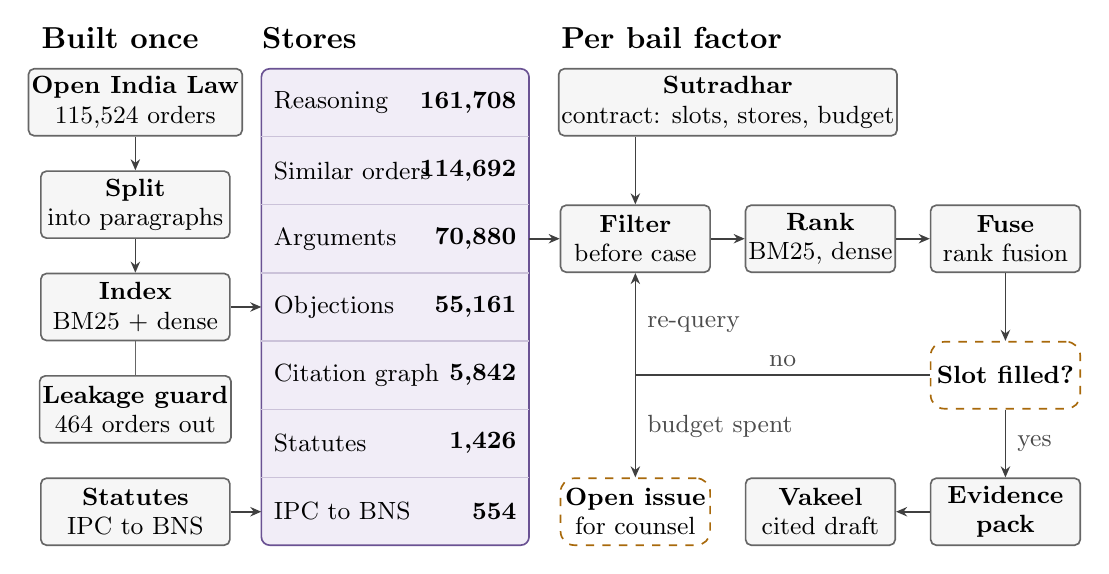
\begin{tikzpicture}[
  font=\fontsize{9}{10.5}\selectfont, line width=0.6pt,
  >={Stealth[length=4pt,width=3.4pt]},
  bx/.style={draw=black!60, fill=bxF, rounded corners=2pt, align=center, inner sep=1pt, minimum height=0.85cm},
  dc/.style={draw=gtD, dashed, fill=white, rounded corners=5pt, align=center, inner sep=1pt, minimum height=0.85cm},
  ar/.style={->, draw=black!75},
  lb/.style={text=black!70, inner sep=1pt},
  ttl/.style={font=\fontsize{10.5}{12}\selectfont\bfseries, anchor=base west, inner sep=0pt}]
% ---- grid ----------------------------------------------------------------
% built-once column x in [0, 2.4]; stores x in [2.8, 6.2]; factor columns centred at 7.55, 9.9, 12.25
% built-once rows every 1.3 cm; factor rows every 1.733 cm; both span y = -0.8 to -6.0
\def\bw{2.4}\def\fw{1.9}
\def\cA{7.55}\def\cB{9.9}\def\cC{12.25}
\def\rA{-0.8}\def\rB{-2.533}\def\rC{-4.267}\def\rD{-6.0}
% ---- titles ----------------------------------------------------------------
\node[ttl] at (0,-0.12) {Built once};
\node[ttl] at (2.8,-0.12) {Stores};
\node[ttl] at (6.6,-0.12) {Per bail factor};
% ---- built once ------------------------------------------------------------
\node[bx, minimum width=\bw cm] (oil) at (1.2,-0.8) {\textbf{Open India Law}\\115,524 orders};
\node[bx, minimum width=\bw cm] (sp)  at (1.2,-2.1) {\textbf{Split}\\into paragraphs};
\node[bx, minimum width=\bw cm] (ix)  at (1.2,-3.4) {\textbf{Index}\\BM25 + dense};
\node[bx, minimum width=\bw cm] (lk)  at (1.2,-4.7) {\textbf{Leakage guard}\\464 orders out};
\node[bx, minimum width=\bw cm] (stt) at (1.2,-6.0) {\textbf{Statutes}\\IPC to BNS};
\draw[ar] (oil) -- (sp);
\draw[ar] (sp) -- (ix);
\draw[draw=black!60] (ix) -- (lk);
% ---- stores ----------------------------------------------------------------
\def\sL{2.8}\def\sR{6.2}\def\sT{-0.375}\def\sB{-6.425}
\draw[draw=stD, fill=stF, rounded corners=3pt] (\sL,\sT) rectangle (\sR,\sB);
\foreach \i/\n/\c in {0/Reasoning/{161,708}, 1/Similar orders/{114,692}, 2/Arguments/{70,880},
                      3/Objections/{55,161}, 4/Citation graph/{5,842}, 5/Statutes/{1,426}, 6/IPC to BNS/{554}} {
  \pgfmathsetmacro{\y}{\sT+(\i+0.5)*(\sB-\sT)/7}
  \node[anchor=west, inner sep=0pt] at (\sL+0.15,\y) {\n};
  \node[anchor=east, inner sep=0pt] at (\sR-0.15,\y) {\textbf{\c}};
}
\foreach \i in {1,...,6} {
  \pgfmathsetmacro{\y}{\sT+\i*(\sB-\sT)/7}
  \draw[draw=stD!35, line width=0.4pt] (\sL,\y) -- (\sR,\y);
}
\draw[ar] (ix.east) -- (\sL,-3.4);
\draw[ar] (stt.east) -- (\sL,-6.0);
% ---- per bail factor -------------------------------------------------------
\node[bx, minimum width=4.25cm] (su) at ({(\cA+\cB)/2},\rA) {\textbf{Sutradhar}\\contract: slots, stores, budget};
\node[bx, minimum width=\fw cm] (fi) at (\cA,\rB) {\textbf{Filter}\\before case};
\node[bx, minimum width=\fw cm] (rk) at (\cB,\rB) {\textbf{Rank}\\BM25, dense};
\node[bx, minimum width=\fw cm] (fu) at (\cC,\rB) {\textbf{Fuse}\\rank fusion};
\node[dc, minimum width=\fw cm] (q)  at (\cC,\rC) {\textbf{Slot filled?}};
\node[bx, minimum width=\fw cm] (ep) at (\cC,\rD) {\textbf{Evidence}\\\textbf{pack}};
\node[bx, minimum width=\fw cm] (va) at (\cB,\rD) {\textbf{Vakeel}\\cited draft};
\node[dc, minimum width=\fw cm] (oi) at (\cA,\rD) {\textbf{Open issue}\\for counsel};
\draw[ar] (\sR,\rB) -- (fi.west);
\draw[ar] (su.south -| fi.north) -- (fi.north);
\draw[ar] (fi) -- (rk);
\draw[ar] (rk) -- (fu);
\draw[ar] (fu) -- (q);
\draw[ar] (q) -- node[lb, right=3pt] {yes} (ep);
\draw[ar] (ep) -- (va);
\draw[draw=black!75] (q.west) -- node[lb, above=2pt] {no} (\cA,\rC);
\draw[ar] (\cA,\rC) -- node[lb, right=3pt] {re-query} (fi.south);
\draw[ar] (\cA,\rC) -- node[lb, right=3pt] {budget spent} (oi.north);
\end{tikzpicture}
\end{document}
